\subsubsection{List (mutable)}
\begin{itemize}
    \item ordered data
    \item Fast Access via index
    \item Slow for updates
\end{itemize}

{\centering\underline{\textbf{Initialise a list with []}} \par}
\begin{lstlisting}
l = [1, 3, "hi", -4]
M = [[-1 for i in range(n)] for j in range(m)]
# 2D list or m x n-Matrix filled with -1
\end{lstlisting}

{\centering\underline{\textbf{Common List Operations}} \par}
\lstinputlisting{src/3_containers/code/2_2_list_operation.py}

{\centering\underline{\textbf{List Comprehension}} \par}
Apply a function $f(x)$ to all items in list l:
\begin{lstlisting}
l2 = [f(x) for x in l] #z.g. 2*x for f(x)
\end{lstlisting}
Apply a function $f(x)$ to a range:
\begin{lstlisting}
r2 = [f(x) for x in range(1,6)]
\end{lstlisting}
Apply a function $f(x)$ only to items in list l that satisfy $g(x)$ (filter):
\begin{lstlisting}
l3 = [f(x) for x in l if g(x)]
\end{lstlisting}
Example: Read a sequence of numbers:
\begin{lstlisting}
l = [int(x) for x in input("Input: ").split()]
\end{lstlisting}

\subsubsection{Sorting Algorithms for Lists} \label{section_sorting_list}
    {\centering\underline{\textbf{Selection Sort}} \par}
        \begin{minipage}{0.59\linewidth}
            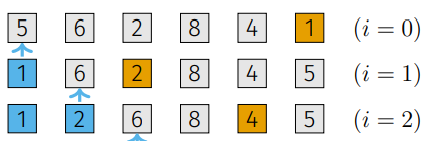
\includegraphics[width = \linewidth]{src/3_containers/images/selection_sort.png}
        \end{minipage}
        \begin{minipage}{0.39\linewidth}
            \fcolorbox{black}{cyan}{sorted list}\\
            \fcolorbox{black}{white}{unsorted list}\\
            \fcolorbox{black}{orange}{smallest value}
        \end{minipage}

        \lstinputlisting{src/3_containers/code/2_2_1_selection_sort.py}

    {\centering\underline{\textbf{Insertion Sort}} \par}
        \begin{minipage}{0.64\linewidth}
            \lstinputlisting{src/3_containers/code/2_2_1_insertion_sort.py}
        \end{minipage}
        \begin{minipage}{0.34\linewidth}
            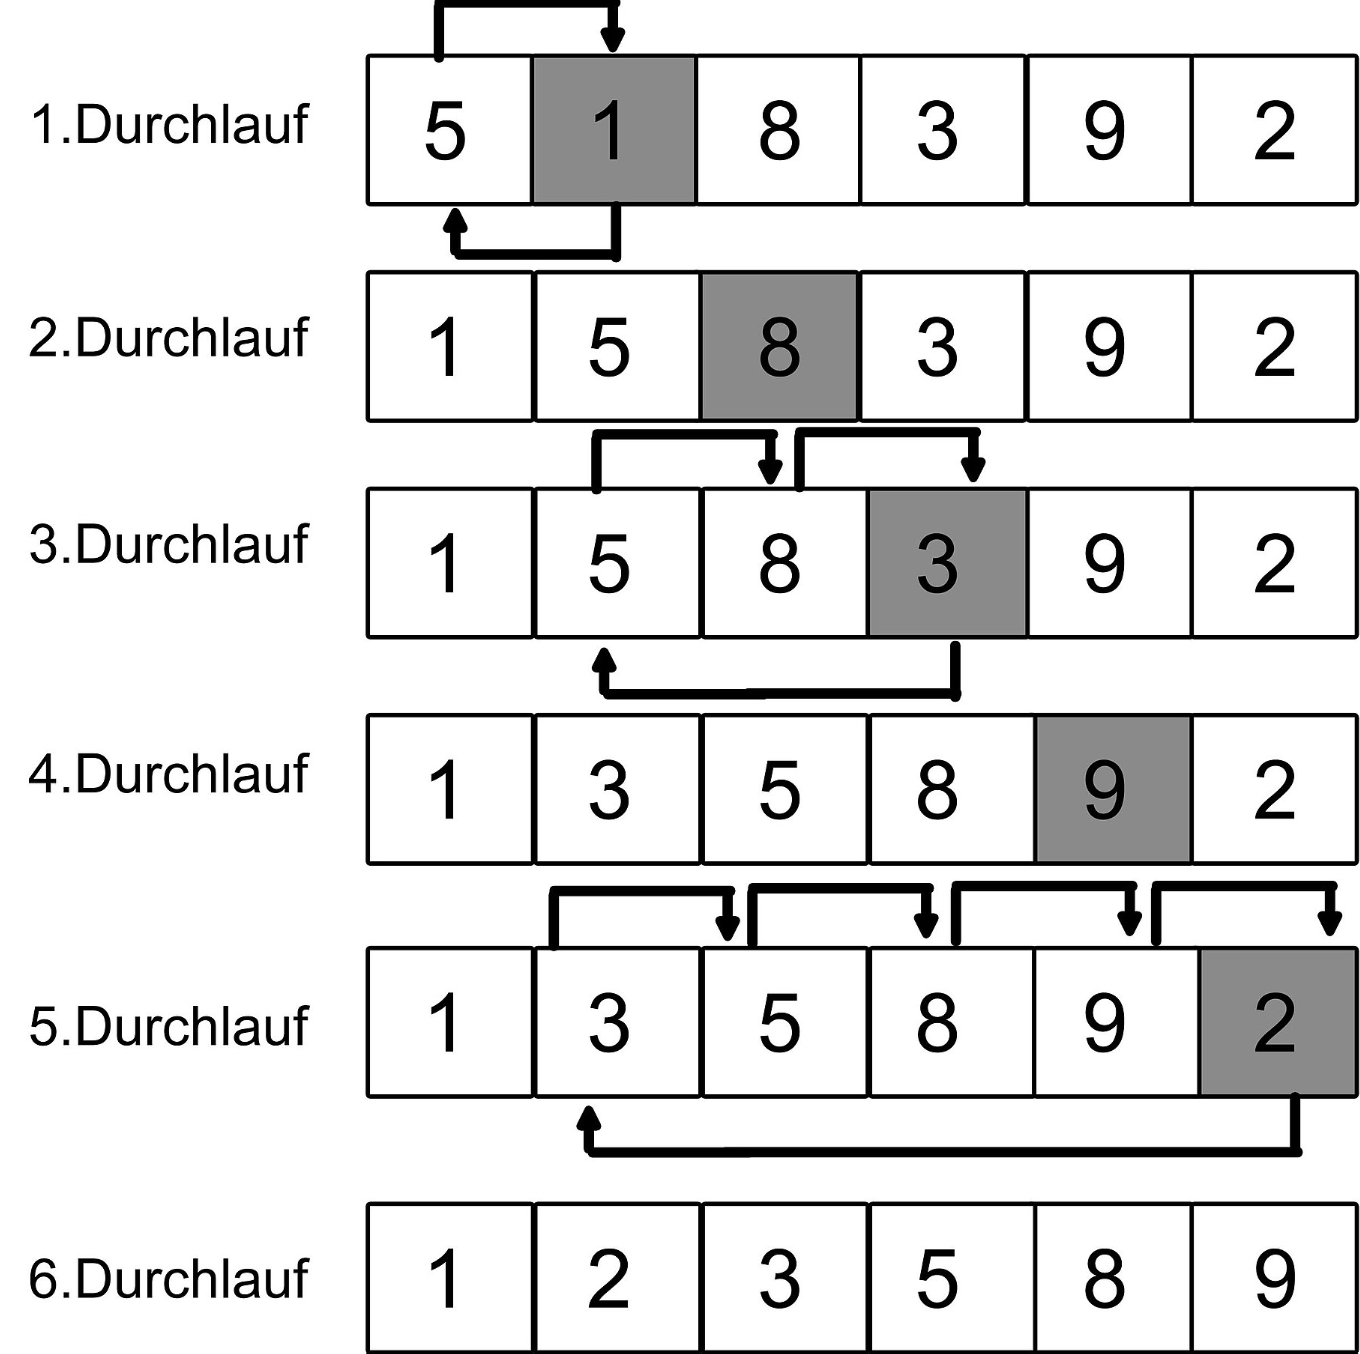
\includegraphics[width = \linewidth]{src/3_containers/images/insertion_sort.png}
        \end{minipage}

    {\centering\underline{\textbf{Bubble Sort}} \par}
        {\centering \includegraphics*[width = 0.8\linewidth]{src/3_containers/images/bubble_sort.png} \par}
        \lstinputlisting{src/3_containers/code/2_2_1_bubble_sort.py}
        
    {\centering\underline{\textbf{Mergesort (Divide and Conquer)}} \par}
        Requires $\Theta(n)$ additional storage\\
        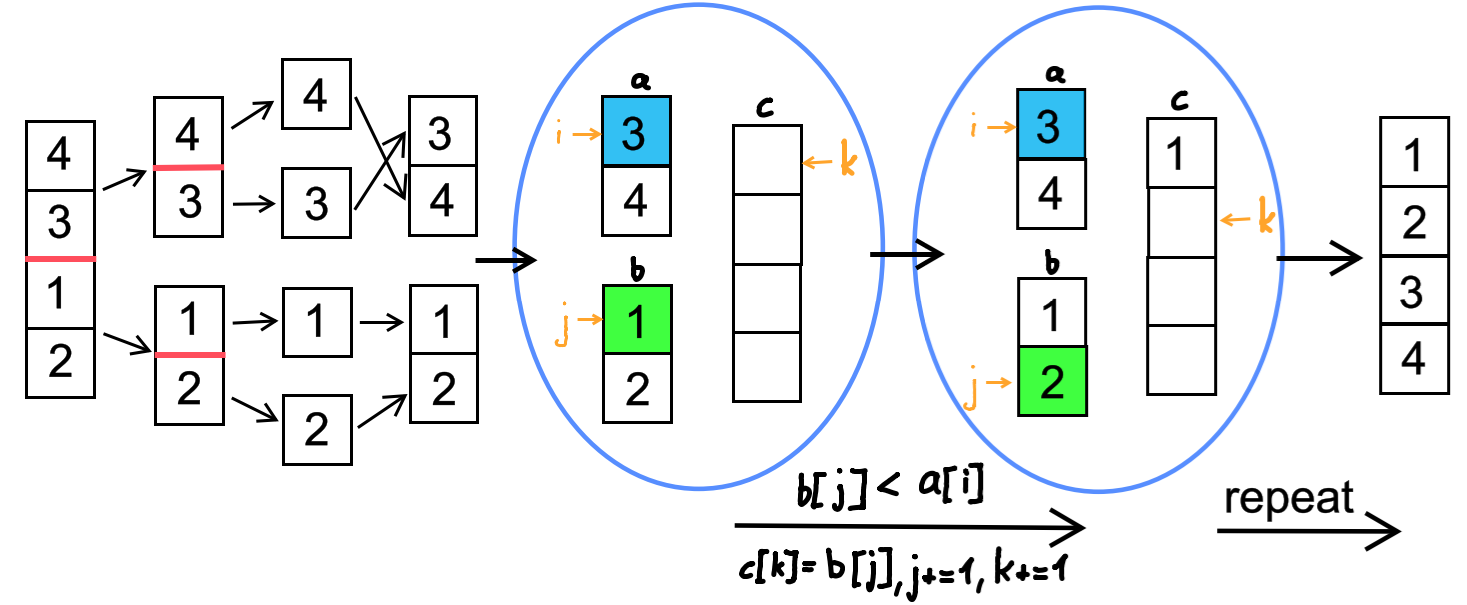
\includegraphics[width = \linewidth]{src/3_containers/images/mergesort.png}
        \fcolorbox{black}{cyan}{greater value}  \fcolorbox{black}{green}{smaller value}

        \lstinputlisting{src/3_containers/code/2_2_1_mergesort.py}
    
    {\centering\underline{\textbf{Quick Sort (Divide and Conquer)}} \par}
        Requires no additional storage\\
        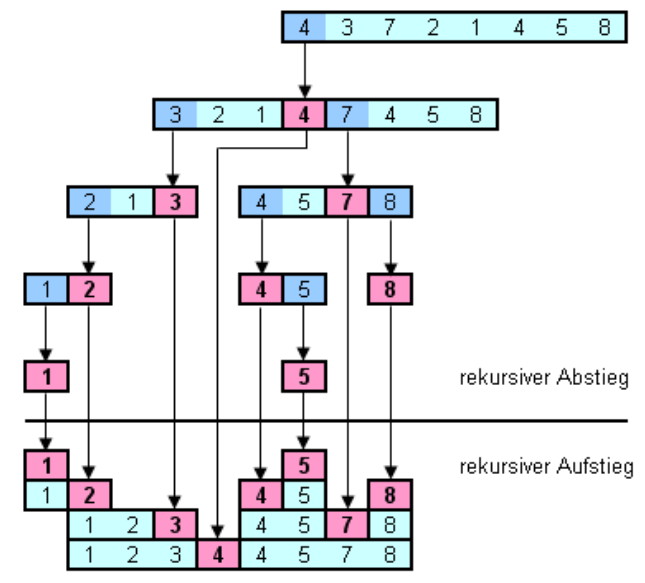
\includegraphics[width = \linewidth]{src/3_containers/images/quicksort.png}
        \fcolorbox{black}{ProcessBlue}{Pivot}  \fcolorbox{black}{CarnationPink}{Pivot is now at correct position}
        \lstinputlisting{src/3_containers/code/2_2_1_quick_sort.py}

\subsubsection{Search Algorithms for Lists}
    {\centering\underline{\textbf{Linear Search}} \par}
        \includegraphics*[width = 0.8\linewidth]{src/3_containers/images/linear_search.png}
        \lstinputlisting{src/3_containers/code/2_2_2_linear_search.py}

    {\centering\underline{\textbf{Binary Search}} \par}
        \includegraphics*[width = 0.8\linewidth]{src/3_containers/images/binary_search.png}
        \lstinputlisting{src/3_containers/code/2_2_2_binary_search.py}
